% File: main.tex
% Date: 2015, April
% Authors: Gustavo Peixoto, Leon Lima.
% Description: Latex template file for seminar short papers presented at PPG-EM/UERJ.
% Version: 1.0
% Available online on: www.gesar.uerj.br

%% PREAMBLE
\documentclass[date]{ppgem} 

%% TITLE
\Title{Preparing your abstract to be presented at PPG-EM's seminars: a
first tutorial}

%% AUTHORS
\AuthorName{César Lattes}
\CorrEmail{lattes@uerj.br}
\AdvisorName{Carlos Chagas}
\CoAdvisorName{} 
\Year{2016}

%% INSTITUTION
\InstA{State University of Rio de Janeiro} 
\InstB{} 

\pagestyle{fancy}
\lhead{\small{Author's Name}}
\rhead{\small{Title or short title}}

\begin{document}
\thispagestyle{plain}
\makeheader

\begin{multicols}{2}

%% KEYWORDS
\begin{keywords}
Max of 4 keywords, comma separeted, {\LaTeX} typesetting, standardisation.
\end{keywords}

%% BODY
\section{Introduction}

This short paper is intended to introduce a self-explained tutorial on
how to prepare abstract texts to be presented in the form of internal
seminars at Graduate Program in Mechanical Engineering (now on PPG-EM),
from State University of Rio de Janeiro (UERJ). In order to suggest a
standard formatting for better organization and registration at PPG-EM
as well as to help incoming students to be acquainted with the {\LaTeX}
typesetting, this paper also dismembers into a few goals, such as: i) to
work as an introductory text for training in scientific writing among
the PPG-EM's students and seminar attendees; ii) to strengthen the
practical use of English language over the academic environment; iii) to
provide guidelines to outline the first versions of those research
issues that will may be turned into extended abstracts and/or conference
papers, and iv) to enhance the PPG-EM's academic competitiveness
worldwide. 

\section{Text elements and organization}

Basically, your paper should have five major parts: i) Introduction; ii)
Methodology; iii) Results; iv) Discussion and v) Conclusion, although
the parts iv) e v) may be combined into a unique section. 

You are free to set out the title of your paper provided that you have
good reasons to support your choice. It should be totally capitalised.
All the sections and subsections should have only the first letter
capitalised, except when a proper noun is required. The following
example could be used for titles:

\begin{itemize}
\item CONTINUUM MECHANICS BOOKSHELF: FROM TRUESDELL TO MASE, 
\end{itemize}
whereas
\begin{itemize}
\item  Supercritical flows for $ 10 < Fr < 100 $, \\
\item  Physicochemistry of copper nanoparticules  \\
\end{itemize}

could be applied to sections or subsections. 

\section{Model and data presentation}

This section explains how to insert equations, figures and tables into
your text as well as references to them.

\subsection{Equations \label{subsec:eqs}}

If you need to write equations in your text, whether to represent a
model based on differential equations, whether to define expressions of
lower complexity, the usual {\LaTeX} environments are applicable to
whatever you intend to do, \textit{e.g.} a uniquely labelled equation

\begin{equation}
\label{eq:1}
  \frac{L}{A}\frac{dW}{dt}=\rho_0\beta g\oint Tdz-f\frac{L}{D}\frac{W^2}{2\rho_0A^2}
\end{equation}

or multi-line labelled equations like 

\begin{subequations}
\label{eq:2}
\begin{eqnarray}
\frac{\D T_1}{\D t}+\frac{W}{A\rho_0}\frac{\D T_1}{\D s}&=&\frac{4q}{D\rho_1c_p} \label{eq:2a} \\
\frac{\D T_2}{\D t}+\frac{W}{A\rho_1}\frac{\D T_2}{\D s}&=&-\frac{4U(\overline{T}-T_s)}{D\rho_2c_p} \label{eq:2b} \\
\frac{\D T_3}{\D t}+\frac{W}{A\rho_2}\frac{\D T_3}{\D s}&=& \displaystyle \sum_{n=-\infty}^{\infty} \sin(n \lambda_3)T_3 \label{eq:2c}
 \end{eqnarray}
\end{subequations}

or

\begin{eqnarray}
\label{eq:3}
  f &=& 8\left[\left(\frac{8}{\Re}\right)^{12} + (A+B^{-1,5})\right]^{1/12} \nonumber \\
  A &=& \left\{-2,457\ln\left[\left(\frac{7}{\Re}\right)^{0,9} + \frac{0,27e}{D}\right]\right\}^{16} \\
  B &=& \left(\frac{37530}{\Re}\right)^{16} \nonumber.
\end{eqnarray}

To reference equations, you may use the commands \verb|\ref{<ref>}| or
\verb|\eqref{<ref>}|. ``Equation \eqref{eq:1}'' is the way how you
should refer to an equation at the beginning of a statement. ``Equations
(\ref{eq:2a}-\ref{eq:2c})'' is the second way, for multi-line cases. If
you need refer to another equation in the middle of the text, then you
should write ``Eq.~(\ref{eq:2a}-\ref{eq:2c})'' or just
``Eq.~\eqref{eq:3}''.

\subsection{Figures}

Figures are added to your paper as a \emph{nonfloat} element by calling

\begin{verbatim}
 \begin{center}\includegraphics[...]
 {figs/<fig_name>} 
 (...)
 \end{center}
\end{verbatim}

so that such a figure...

\begin{center}
 \captionsetup{type=figure}
 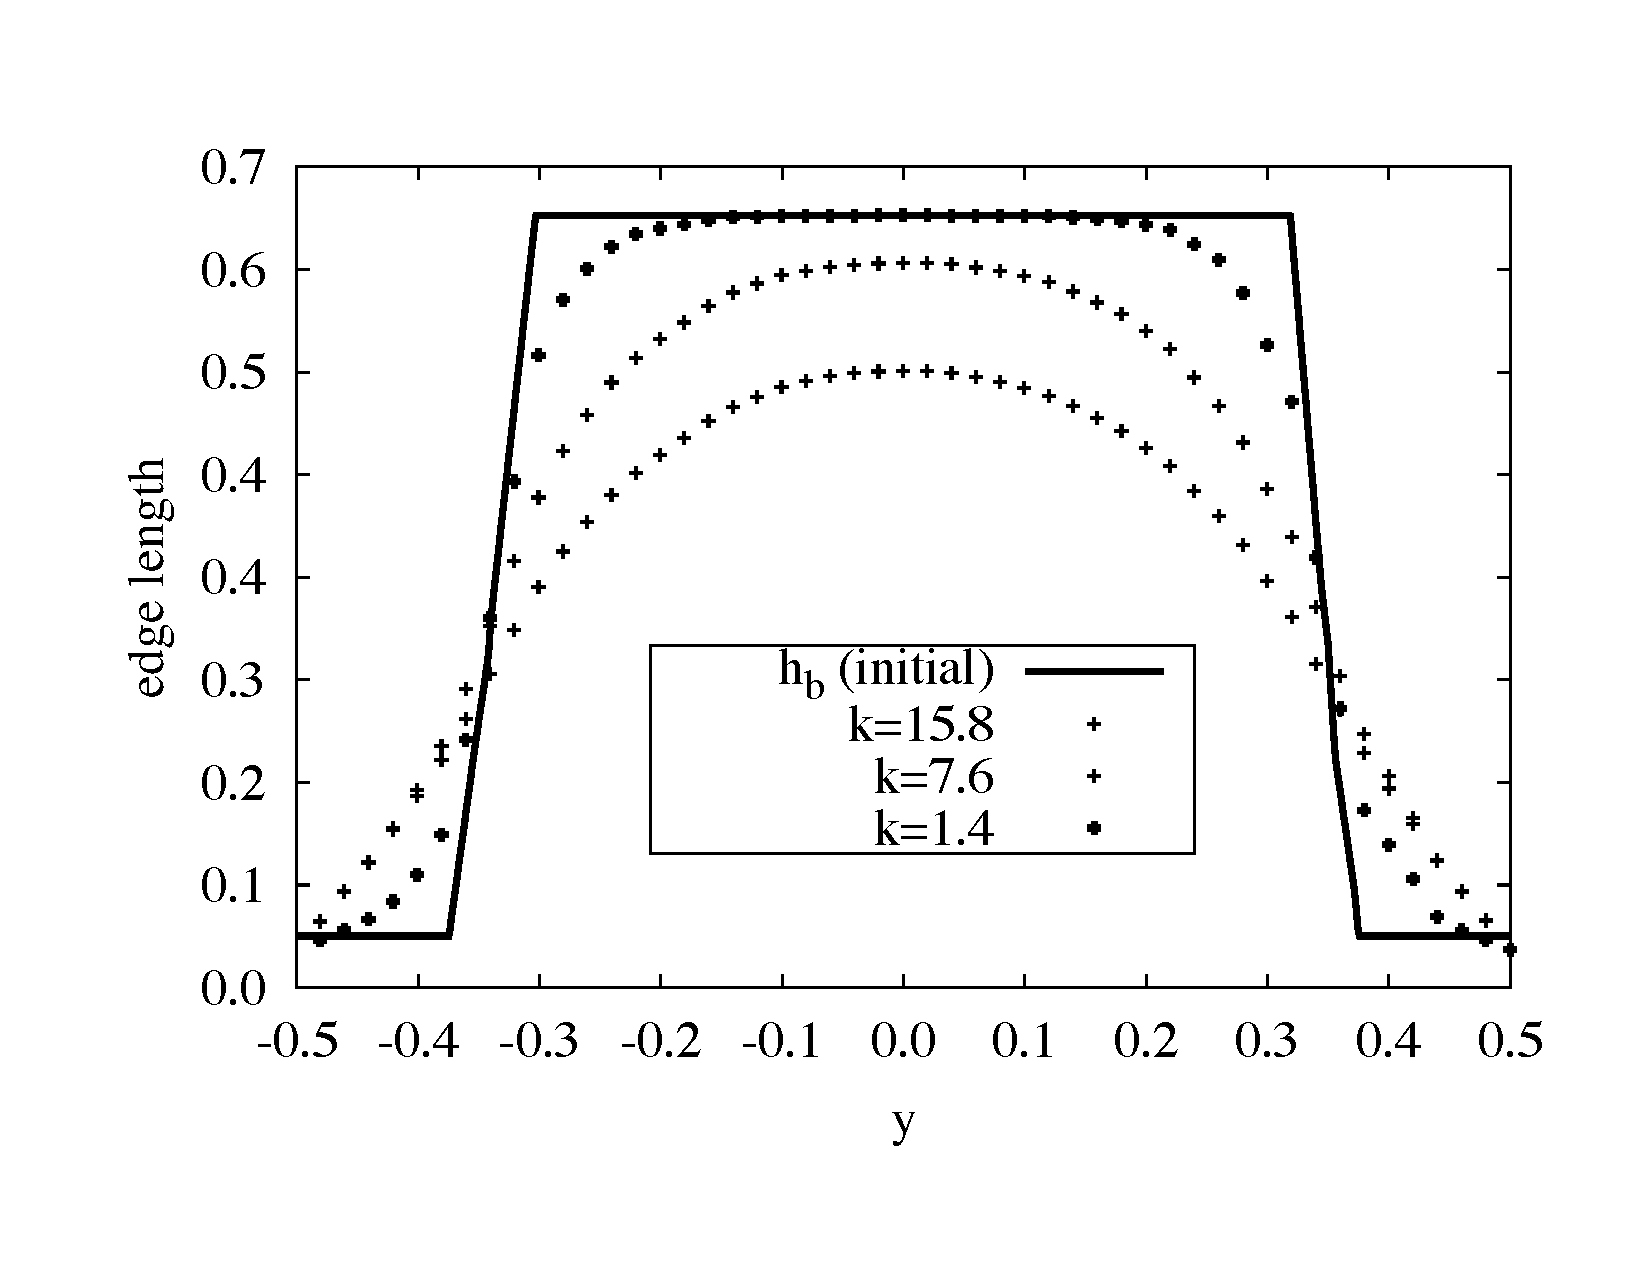
\includegraphics[scale=0.33]{figs/example}
 \figcaption{Solutions of the Helmholtz’s equations for different
 diffusive parameter k}
 \label{fig:mass-flow}
\end{center}

...is a good example of well placed figure. Reference to figures follow
the examples given in Subsection~\ref{subsec:eqs}. That is to say,
``Figure \eqref{fig:mass-flow}'' is the way how you should refer to a
figure at the beginning of a statement. If you need refer to a figure in
the middle of the text, then you should write
``Fig.~\ref{fig:mass-flow}''. In this case, parentheses are not
required.

\subsection{Tables}

Tables like \ref{tbl:1} can also be inserted into your text through the
environment \verb|tabular|.

\begin{center}
  \captionsetup{type=table}
  \begin{tabular}{ccc}
    \hline
    & lower bound & upper bound\\
    \hline
    \citet{ambrosini2004} & 285 W & 480 W\\
    present model & 390 W & 707 W\\
    \hline\\
  \end{tabular}
  \tabcaption{Stability thresholds using Churchill's friction
  correlation, with external fluid temperature of 30ºC.}
  \label{tbl:1}
\end{center}

Reference to tables should not be abbreviated. That is to say, ``Table
\ref{tbl:1}'' is the way how you should refer to a figure both at the
beginning and in the middle of a statement. Parentheses are not required
here as well. \subsection{Citations}

To cite other authors or references, use the textual and parenthetical
commands provided by \verb|natbib| package \verb|\cite{<ref1>}| or
\verb|\citep{<ref1>}|. Add your references to the file \verb|refs.bib|
and compile the document by calling \verb|bibtex|. The usual \verb|bib|
entries are available (see file \verb|refs.bib| in the root directory).
This paper's bibliography, for instance, is formed by: a M.Sc. thesis
\citep{rabellomsc2007}, a tech report \cite{amarante2001}, a book
\citep{batchelor1994}, an inproceedings \cite{lima2009}, a Ph.D. thesis
\citep{loureirophd2008} and a miscellaneous-like reference
\citep{mangiavacchi2000}.

\section{Conclusions}

Here, you will end up your text by drawing conclusions and comments
about future work. In order to reduce the contents, we encourage you to
summarize the main results by using an itemised list as follows:

\begin{itemize}
 \item this tutorial has discussed the PPG-EM's paper template;
 \item the usability of {\LaTeX} typesetting was presented;
 \item a standard template for internal seminars was suggested;
 \item to develop other presentation templates is a future goal. 
\end{itemize}

\section{Acknowledgments}

(This section is optional). However, a simple remark like ``The authors
thank to Prof. Gustavo R. dos Anjos for sharing insights and ideas in
developing the PPG-EM's academic templates.'' may be included. 

%% REFERENCES
\bibliographystyle{plainnat}
\bibliography{refs}

\end{multicols}
\end{document}
